

\tikzset{every picture/.style={line width=0.75pt}} %set default line width to 0.75pt        

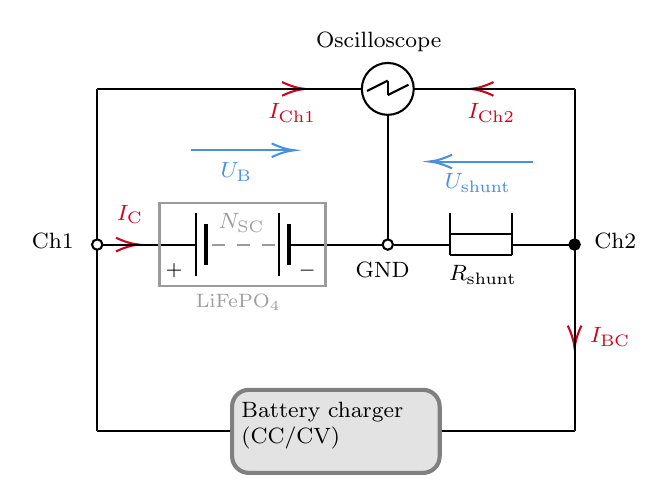
\begin{tikzpicture}[x=0.75pt,y=0.75pt,yscale=-1,xscale=1]
%uncomment if require: \path (0,748); %set diagram left start at 0, and has height of 748

%Straight Lines [id:da030470885996142894] 
\draw [color={rgb, 255:red, 208; green, 2; blue, 27 }  ,draw opacity=1 ]   (360,170) ;
\draw [shift={(360,170)}, rotate = 180] [color={rgb, 255:red, 208; green, 2; blue, 27 }  ,draw opacity=1 ][line width=0.75]    (10.93,-3.29) .. controls (6.95,-1.4) and (3.31,-0.3) .. (0,0) .. controls (3.31,0.3) and (6.95,1.4) .. (10.93,3.29)   ;
%Straight Lines [id:da3824823238969528] 
\draw [color={rgb, 255:red, 208; green, 2; blue, 27 }  ,draw opacity=1 ]   (570,205) -- (570,218) ;
\draw [shift={(570,220)}, rotate = 270] [color={rgb, 255:red, 208; green, 2; blue, 27 }  ,draw opacity=1 ][line width=0.75]    (10.93,-3.29) .. controls (6.95,-1.4) and (3.31,-0.3) .. (0,0) .. controls (3.31,0.3) and (6.95,1.4) .. (10.93,3.29)   ;
%Straight Lines [id:da5182691574210985] 
\draw    (340,260) -- (407.5,260) ;
%Straight Lines [id:da26468661252829784] 
\draw    (502.5,260) -- (570,260) ;
%Rounded Rect [id:dp15109738720083965] 
\draw  [color={rgb, 255:red, 128; green, 128; blue, 128 }  ,draw opacity=1 ][fill={rgb, 255:red, 227; green, 227; blue, 227 }  ,fill opacity=1 ][line width=1.5]  (405,248) .. controls (405,243.58) and (408.58,240) .. (413,240) -- (497,240) .. controls (501.42,240) and (505,243.58) .. (505,248) -- (505,272) .. controls (505,276.42) and (501.42,280) .. (497,280) -- (413,280) .. controls (408.58,280) and (405,276.42) .. (405,272) -- cycle ;
%Straight Lines [id:da04571217565366692] 
\draw [color={rgb, 255:red, 208; green, 2; blue, 27 }  ,draw opacity=1 ]   (535,95) -- (522,95) ;
\draw [shift={(520,95)}, rotate = 360] [color={rgb, 255:red, 208; green, 2; blue, 27 }  ,draw opacity=1 ][line width=0.75]    (10.93,-3.29) .. controls (6.95,-1.4) and (3.31,-0.3) .. (0,0) .. controls (3.31,0.3) and (6.95,1.4) .. (10.93,3.29)   ;
%Straight Lines [id:da286200132644544] 
\draw    (342,170) -- (370,170) ;
%Straight Lines [id:da17958881147308237] 
\draw    (450.5,170) -- (477.5,170) ;
%Straight Lines [id:da5043205087506204] 
\draw [color={rgb, 255:red, 208; green, 2; blue, 27 }  ,draw opacity=1 ]   (425,95) -- (438,95) ;
\draw [shift={(440,95)}, rotate = 180] [color={rgb, 255:red, 208; green, 2; blue, 27 }  ,draw opacity=1 ][line width=0.75]    (10.93,-3.29) .. controls (6.95,-1.4) and (3.31,-0.3) .. (0,0) .. controls (3.31,0.3) and (6.95,1.4) .. (10.93,3.29)   ;
%Straight Lines [id:da8819726416071505] 
\draw [line width=0.75]    (387.5,155) -- (387.5,185) ;
%Straight Lines [id:da22364644407030787] 
\draw [color={rgb, 255:red, 155; green, 155; blue, 155 }  ,draw opacity=1 ] [dash pattern={on 4.5pt off 4.5pt}]  (425.5,170) -- (390.5,170) ;
%Straight Lines [id:da8171048209291414] 
\draw [line width=1.5]    (392.5,160) -- (392.5,180) ;
%Straight Lines [id:da3784748951709651] 
\draw [line width=0.75]    (427.5,155) -- (427.5,185) ;
%Straight Lines [id:da23453075334713613] 
\draw [line width=1.5]    (432.5,160) -- (432.5,180) ;
%Straight Lines [id:da7174267672251604] 
\draw    (387.5,170) -- (370.5,170) ;
%Straight Lines [id:da8824908036219616] 
\draw    (449.5,170) -- (432.5,170) ;
%Shape: Rectangle [id:dp6355233140968859] 
\draw  [color={rgb, 255:red, 155; green, 155; blue, 155 }  ,draw opacity=1 ] (450,150) -- (450,190) -- (370,190) -- (370,150) -- cycle ;
%Shape: Circle [id:dp4046675137999993] 
\draw   (477.5,170) .. controls (477.5,168.62) and (478.62,167.5) .. (480,167.5) .. controls (481.38,167.5) and (482.5,168.62) .. (482.5,170) .. controls (482.5,171.38) and (481.38,172.5) .. (480,172.5) .. controls (478.62,172.5) and (477.5,171.38) .. (477.5,170) -- cycle ;
%Shape: Circle [id:dp8699232468402804] 
\draw   (337.5,170) .. controls (337.5,168.62) and (338.62,167.5) .. (340,167.5) .. controls (341.38,167.5) and (342.5,168.62) .. (342.5,170) .. controls (342.5,171.38) and (341.38,172.5) .. (340,172.5) .. controls (338.62,172.5) and (337.5,171.38) .. (337.5,170) -- cycle ;
%Straight Lines [id:da0932789662810869] 
\draw    (340,95) -- (340,167.5) ;
%Straight Lines [id:da7259313392072295] 
\draw    (340,95) -- (467.5,95) ;
%Straight Lines [id:da7181235672344906] 
\draw [color={rgb, 255:red, 74; green, 144; blue, 226 }  ,draw opacity=1 ]   (385,124.57) -- (433,124.57) ;
\draw [shift={(435,124.57)}, rotate = 180] [color={rgb, 255:red, 74; green, 144; blue, 226 }  ,draw opacity=1 ][line width=0.75]    (10.93,-3.29) .. controls (6.95,-1.4) and (3.31,-0.3) .. (0,0) .. controls (3.31,0.3) and (6.95,1.4) .. (10.93,3.29)   ;
%Shape: Circle [id:dp9954794574731103] 
\draw   (467.5,95) .. controls (467.5,88.1) and (473.1,82.5) .. (480,82.5) .. controls (486.9,82.5) and (492.5,88.1) .. (492.5,95) .. controls (492.5,101.9) and (486.9,107.5) .. (480,107.5) .. controls (473.1,107.5) and (467.5,101.9) .. (467.5,95) -- cycle ;
%Straight Lines [id:da04493405460274014] 
\draw    (470,96) -- (480,91) ;
%Straight Lines [id:da3033269159759058] 
\draw    (480,91) -- (480,98) ;
%Straight Lines [id:da8245646456208624] 
\draw    (480,98) -- (490,93) ;

%Straight Lines [id:da664654756239323] 
\draw    (340,172.5) -- (340,260) ;
%Straight Lines [id:da020631229787501093] 
\draw    (570,170) -- (570,260) ;
%Straight Lines [id:da42439143356479936] 
\draw    (492.5,95) -- (570,95) ;
%Straight Lines [id:da8878395010937925] 
\draw    (540,175) -- (540,165) ;
%Straight Lines [id:da5068559712609504] 
\draw    (510,175) -- (510,165) ;
%Straight Lines [id:da17027035780260014] 
\draw    (510,175) -- (540,175) ;
%Straight Lines [id:da7267594413628695] 
\draw    (510,165) -- (540,165) ;
%Straight Lines [id:da6452827698871475] 
\draw    (510,155) -- (510,165) ;
%Straight Lines [id:da9670069496965643] 
\draw    (540,155) -- (540,165) ;
%Shape: Circle [id:dp9967471299276287] 
\draw  [fill={rgb, 255:red, 0; green, 0; blue, 0 }  ,fill opacity=1 ] (570,167.5) .. controls (571.38,167.5) and (572.5,168.62) .. (572.5,170) .. controls (572.5,171.38) and (571.38,172.5) .. (570,172.5) .. controls (568.62,172.5) and (567.5,171.38) .. (567.5,170) .. controls (567.5,168.62) and (568.62,167.5) .. (570,167.5) -- cycle ;
%Straight Lines [id:da6778579527436412] 
\draw    (540,170) -- (570,170) ;
%Straight Lines [id:da9391362233033829] 
\draw    (483,170) -- (510,170) ;
%Straight Lines [id:da8151174249515367] 
\draw    (480,107.5) -- (480,167.5) ;
%Straight Lines [id:da4990891660653225] 
\draw [color={rgb, 255:red, 74; green, 144; blue, 226 }  ,draw opacity=1 ]   (550,130) -- (502,130) ;
\draw [shift={(500,130)}, rotate = 360] [color={rgb, 255:red, 74; green, 144; blue, 226 }  ,draw opacity=1 ][line width=0.75]    (10.93,-3.29) .. controls (6.95,-1.4) and (3.31,-0.3) .. (0,0) .. controls (3.31,0.3) and (6.95,1.4) .. (10.93,3.29)   ;
%Straight Lines [id:da37596819517946445] 
\draw    (570,95) -- (570,167.5) ;

% Text Node
\draw (576,208.4) node [anchor=north west][inner sep=0.75pt]  [font=\footnotesize,color={rgb, 255:red, 208; green, 2; blue, 27 }  ,opacity=1 ]  {$I_{\mathrm{BC}}$};
% Text Node
\draw (348,149.4) node [anchor=north west][inner sep=0.75pt]  [font=\footnotesize,color={rgb, 255:red, 208; green, 2; blue, 27 }  ,opacity=1 ]  {$I_{\mathrm{C}}$};
% Text Node
\draw (408,244.5) node [anchor=north west][inner sep=0.75pt]  [font=\footnotesize] [align=left] {Battery charger\\(CC/CV)};
% Text Node
\draw (386,192.4) node [anchor=north west][inner sep=0.75pt]  [font=\scriptsize,color={rgb, 255:red, 0; green, 0; blue, 0 }  ,opacity=1 ]  {$\mathrm{\textcolor[rgb]{0.61,0.61,0.61}{LiFePO}\textcolor[rgb]{0.61,0.61,0.61}{_{4}}}$};
% Text Node
\draw (435.5,177.4) node [anchor=north west][inner sep=0.75pt]  [font=\scriptsize]  {$-$};
% Text Node
\draw (371.5,177.4) node [anchor=north west][inner sep=0.75pt]  [font=\scriptsize]  {$+$};
% Text Node
\draw (397,153.4) node [anchor=north west][inner sep=0.75pt]  [font=\footnotesize,color={rgb, 255:red, 155; green, 155; blue, 155 }  ,opacity=1 ]  {$N_{\mathrm{SC}}$};
% Text Node
\draw (398,128.97) node [anchor=north west][inner sep=0.75pt]  [font=\footnotesize,color={rgb, 255:red, 74; green, 144; blue, 226 }  ,opacity=1 ]  {$U_{\mathrm{B}}$};
% Text Node
\draw (421,100.4) node [anchor=north west][inner sep=0.75pt]  [font=\footnotesize,color={rgb, 255:red, 208; green, 2; blue, 27 }  ,opacity=1 ]  {$I_{\mathrm{Ch} 1}$};
% Text Node
\draw (444,66) node [anchor=north west][inner sep=0.75pt]  [font=\footnotesize] [align=left] {Oscilloscope};
% Text Node
\draw (508,178.4) node [anchor=north west][inner sep=0.75pt]  [font=\footnotesize]  {$R_{\mathrm{shunt}}$};
% Text Node
\draw (506,134.4) node [anchor=north west][inner sep=0.75pt]  [font=\footnotesize,color={rgb, 255:red, 74; green, 144; blue, 226 }  ,opacity=1 ]  {$U_{\mathrm{shunt}}$};
% Text Node
\draw (517,100.4) node [anchor=north west][inner sep=0.75pt]  [font=\footnotesize,color={rgb, 255:red, 208; green, 2; blue, 27 }  ,opacity=1 ]  {$I_{\mathrm{Ch} 2}$};
% Text Node
\draw (463,177) node [anchor=north west][inner sep=0.75pt]  [font=\footnotesize] [align=left] {GND};
% Text Node
\draw (578,163) node [anchor=north west][inner sep=0.75pt]  [font=\footnotesize] [align=left] {Ch2};
% Text Node
\draw (307,163) node [anchor=north west][inner sep=0.75pt]  [font=\footnotesize] [align=left] {Ch1};


\end{tikzpicture}
